\section{可視化表示の仕組みの抽象化}

前章では,トレースログを一般化し,標準形式トレースログとして定義した.
TLVの可視化表示の仕組みは,この標準形式トレースログに依存するように設計されている.
本節では,可視化表現と可視化表現とトレースログの対応を抽象化について述べる.

\subsection{可視化表現}
\label{subsec:visualization}

TLVにおいて,トレースログの可視化表現は,x軸を時系列とした2次元直交座標系における図形の描画であるとした.
本小節では,座標系と図形について詳述する.

\subsubsection{座標系}

図形を定義する座標系と,表示する座標系は分離して考えるとする.
これにより,図形を表示環境から独立して定義することが可能になる.
図形を定義する座標系をローカル座標系,表示する座標系をデバイス座標系と呼称する.

また,TLVでは,高さと時間を次元に持つ,ワールド座標系という座標系を導入した.
ローカル座標系で定義された図形は,はじめに,ワールド座標系における,図形を表示すべき時間の領域にマッピングされ,これを表示環境に依存するデバイス座標系にマッピングすることで表示する.
これにより,図形の表示領域を,抽象度の高い時刻で指定することが可能になる.
ここで,ローカル座標系からワールド座標系へのマッピングをワールド変換と呼称する.
また,表示する時間の領域を表示期間と呼称する.
表示期間は開始時刻と終了時刻で表される時刻のペアである.

ローカル座標系において,図形の大きさと位置を定義する際は,pixel単位による絶対指定か,ワールド座標系へのマッピング領域に対する割合を\%で指定する相対指定かのいずれかを用いる.

図\ref{fig:coordinate}に座標系の例を,図\ref{fig:worldTransform}にワールド変換の例を示す.

\begin{figure}[tb]
\begin{center}
\includegraphics[scale=0.75]{img/coordinate.eps}
\caption{座標系}
\label{fig:coordinate}
\end{center}
\end{figure}

\begin{figure}[tb]
\begin{center}
\includegraphics[scale=0.75]{img/worldTransform.eps}
\caption{ワールド変換}
\label{fig:worldTransform}
\end{center}
\end{figure}

\subsubsection{基本図形と図形,図形群}
可視化表現は,複数の図形を組み合わせることで実現する.
この際,基本となる図形の単位を基本図形と呼称する.

基本図形として扱える形状は楕円,多角形,四角形,線分,矢印,扇形,文字列の7種類とする.
基本図形は,形状や大きさ,位置,塗りつぶしの色,線の色,線種,透明度などの属性を指定して定義する.

複数の基本図形を仮想的にz軸方向に階層的に重ねたものを,単に図形と呼称し,可視化表現の最小単位とする.
図形は,構成する基本図形を順序付きで指定し,名前をつけて定義する.
図形は名前を用いて参照することができ,その際に引数を与えることができるとする.
この際,引数は,図形を構成する基本図形の,任意の属性に割り当てることを想定している.

複数の図形を仮想的にz軸方向に階層的に重ねたものを図形群と呼称する.
図\ref{fig:shapes}に図形と図形群の例を示す.

\begin{figure}[tb]
\begin{center}
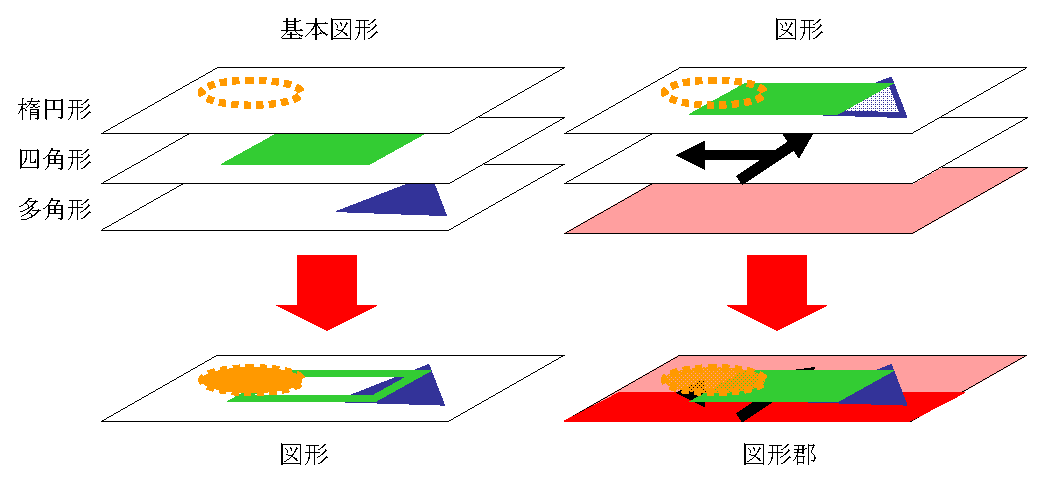
\includegraphics[scale=0.75]{img/shapes.eps}
\caption{図形と図形群}
\label{fig:shapes}
\end{center}
\end{figure}

\subsection{図形とイベントの対応}

本小節では,前小節で述べた可視化表現とトレースログのイベントをどのように対応付けるのかを述べる.

\subsubsection{開始イベント,終了イベント,イベント期間}
前小節において,可視化表現は,図形をワールド変換を経て表示期間にマッピングすることであることを説明した.
ここで,表示期間の開始時刻,終了時刻を,イベントを用いて指定するとする.
つまり,指定されたイベントが発生する時刻をトレースログより抽出することにより表示期間を決定する.
このようにして,トレースログのイベントと可視化表現を対応付ける.
ここで,開始時刻に対応するイベントを開始イベント,終了時刻に対応するイベントを終了イベントと呼称し,表示期間をイベントで表現したものをイベント期間と呼称する.

\subsubsection{可視化ルール}
図形群と,そのマッピング対象であるイベント期間を構成要素としてもつ構造体を,可視化ルールと呼称する.
図\ref{fig:timeShape}に,標準形式トレースログを用いてイベント期間を定義した可視化ルールの例を示す.
\begin{figure}[tb]
\begin{center}
\includegraphics[scale=0.9]{img/timeShape.eps}
\caption{可視化ルール}
\label{fig:timeShape}
\end{center}
\end{figure}
図\ref{fig:timeShape}において,runningShapeを,位置がローカル座標の原点,大きさがワールド座標系のマッピング領域に対して横幅100\%,縦幅80\%の長方形で色が緑色の図形とする.
この図形を,開始イベント\verb|MAIN_TASK.state=RUNNING|,終了イベント\verb|MAIN_TASK.state|となるイベント期間で表示するよう定義したものが可視化ルールtaskBecomeRunningである.
開始イベント\verb|MAIN_TASK.state=RUNNING|は,リソース\verb|MAIN_TASK|の属性\verb|state|の値が\verb|RUNNING|になったことを表し,終了イベント\verb|MAIN_TASK.state|は,リソース\verb|MAIN_TASK|の属性\verb|state|の値が単に変わったことを表している.

taskBecomeRunningを,表\ref{eventTime}に示すトレースログからイベントを抽出して表示期間の時刻を決定し,図形のワールド変換を行った結果が図\ref{fig:timeShape}の右下に示すものである.

\begin{File}{イベント期間を抽出するトレースログ}{eventTime}
[1000]MAIN_TASK.state=RUNNING
[1100]MAIN_TASK.state=WAITING
\end{File}

\section{図形データの生成}

標準形式変換プロセスを経て得られた標準形式トレースログは,可視化ルールを適用され図形データを生成する.
ここで,図形データとは,ワールド変換が行われた全図形のデータを指す.
可視化ルールは可視化ルールファイルとして与えられ,適用する可視化ルールはリソースファイルに記述する.

図形データの生成方法は,標準形式トレースログを一行ずつ可視化ルールのイベント期間と一致するか判断し,一致した場合にその可視化ルールの表示期間をワールド変換先の領域として採用しワールド変換することで行われる.

\subsection{可視化ルールファイル}
\label{visualizeRuleSection}
可視化ルールファイルには,可視化ルールと,図形の定義を記述する.
可視化ルールファイルは,1つのオブジェクトで構成され,オブジェクトのメンバにターゲット毎の変換ルールを記述する.
メンバ名にターゲット名を記述し,値としてオブジェクトを与え,そのオブジェクトに可視化ルールと図形の定義を記述する.

\subsubsection{図形の定義}

図形の定義は,\ref{subsec:visualization}小節にて述べた抽象化した図形を形式化したものである.

図形の定義は{\tt Shapes}というメンバ名の値にオブジェクトとして記述する.
このオブジェクトのメンバ名には図形の名前を記述する.
そして,その値に図形の定義を基本図形の定義の配列として与える.

表\ref{shapeSample}に{\tt toppers}をターゲットとする図形を定義した例を示す.
例では,{\tt runningShapes}と{\tt readyShapes},{\tt svcShapes}の3つの図形を定義している.
{\tt runningShapes}と{\tt readyShapes}は1つの基本図形で構成され,{\tt svcShapes}は3つの基本図形から構成される.

\begin{File}{可視化ルールファイルで図形を定義した例}{shapeSample}
{
  "toppers":{
    "Shapes":{
      "runningShapes":[
        {
          "Type":"Rectangle",
          "Size":"100%,80%",
          "Pen":{"Color":"ff00ff00","Width":1},
          "Fill":"6600ff00"
        }
      ],
      "readyShapes":[
        {
          "Type":"Line",
          "Points":["l(0),80%","r(0),80%"],
          "Pen":{"Color":"ffffaa00","Width":1}
        }
      ],
      "svcShapes":[
        {
          "Type":"Rectangle",
          "Size":"100%,40%",
          "Pen":{"Color":"${ARG0}","Width":1, "DashStyle":"Dash"},
          "Fill":"${ARG0}",
          "Alpha":100
        },
        {
          "Type":"Text",
          "Size":"100%,40%",
          "Font":{"Align":"TopLeft", "Size":7},
          "Text":"${ARG1}"
        },
        {
          "Type":"Text",
          "Size":"100%,40%",
          "Font":{"Align":"BottomRight", "Size":7},
          "Text":"return ${ARG2}"
        }
      ]
    }
  }
}
\end{File}

基本図形の定義に用いるメンバは,基本図形の形状により異なる.
すべての形状に共通なメンバの説明を以下に示す.

\begin{description}
{\nopagebreak
\item[\texttt{Type}] \mbox{}
    \vspace{-1zw}
    \begin{description}
    \setlength{\itemsep}{-1.5\itemsep}
    \item[説明] 図形の形状.必須である.
    \item[値] 文字列("{\tt Rectangle}":長方形,"{\tt Line}":線分,"{\tt Arrow}":矢印,"{\tt Polygon}":多角形,"{\tt Pie}":扇形,"{\tt Ellipse}":楕円形,"{\tt Text}":文字列のいずれか)
    \end{description}
}{\nopagebreak
\item[\texttt{Size}] \mbox{}
    \vspace{-1zw}
    \begin{description}
    \setlength{\itemsep}{-1.5\itemsep}
    \item[説明] 図形のサイズ.省略した場合,値は"\verb|100%,100%|"となる
    \item[値] サイズ指定形式の文字列
    \end{description}
}{\samepage
\item[\texttt{Location}] \mbox{}
    \vspace{-1zw}
    \begin{description}
    \setlength{\itemsep}{-1.5\itemsep}
    \item[説明] 図形の位置.省略した場合,値は"\verb|0,0|"となる
    \item[値] 位置指定形式の文字列
    \end{description}
}
\clearpage
{\nopagebreak
\item[\texttt{Area}] \mbox{}
    \vspace{-1zw}
    \begin{description}
    \setlength{\itemsep}{-1.5\itemsep}
    \item[説明] 図形の表示領域.サイズと位置を同時に指定する.省略した場合は,サイズに{\tt Size}の値が,位置に{\tt Location}の値が設定される.
    \item[値] 文字列2つの配列.1つ目の要素は位置指定形式,2つ目の要素はサイズ指定形式を記述する
    \end{description}
}{\nopagebreak
\item[\texttt{Offset}] \mbox{}
    \vspace{-1zw}
    \begin{description}
    \setlength{\itemsep}{-1.5\itemsep}
    \item[説明] 図形のオフセット.省略した場合,値は"\verb|0,0|"となる
    \item[値] 位置指定形式の文字列
    \end{description}
}
\end{description}

図形のサイズを指定する形式として,サイズ指定形式({\tt ShapeSize})を次のように定めた.

\begin{EBNF}
ShapeSize = Width,",",Height
Width = /-?([1-9][0-9]*)?[0-9](\.[0-9]*)?(%|px)?/
Height = /-?([1-9][0-9]*)?[0-9](\.[0-9]*)?(%|px)?/
\end{EBNF}

\ref{subsec:visualization}小節において,図形の大きさの指定方法として,絶対指定と相対指定の2つの方法を用いることができるとした.
これらは{\tt px}と{\tt \%}という単位を用いることで指定する.
{\tt px}が絶対指定であり,{\tt \%}が相対指定である.
単位を省略した場合は絶対指定されたものとして解釈される.

また,図形の位置を指定する形式として,位置指定形式({\tt ShapeLocation})を次のように定めた.

\begin{EBNF}
ShapeLocation = X,",",Y
X = ("l"|"c"|"r"),"(",Value,")"|Value;
Y = ("t"|"m"|"b"),"(",Value,")"|Value;
Value = /-?([1-9][0-9]*)?[0-9](\.[0-9]*)?(%|px)?/
\end{EBNF}

図形の位置も,サイズと同じように絶対指定と相対指定の両方で指定することができる.
また,指定する際に基準とする位置を"{\it base}\verb|(|{\it value}\verb|)|"として指定できるようにした.
この指定を基準指定と呼ぶ.
ここで,{\it base}は,{\tt X}の指定の場合,{\tt l}か{\tt c}か{\tt r}であり,それぞれ領域の左端,横方向の中央,右端を指す.
また,{\tt Y}の指定の場合は,{\tt t}か{\tt m}か{\tt b}であり,それぞれ領域の上端,縦方向の中央,下端を指す.

相対指定の際に基準指定することにより,同じ位置を様々な記述方法を用いて指定できる.
例えば,{\tt l(100\%)}と{\tt r(0\%)},{\tt c(50\%)}は領域の右端を指定し,{\tt l(50\%)}と{\tt r(-50\%)},{\tt c(0\%)}は領域の横方向の中央を指す.
同じように{\tt b(100\%)}と{\tt t(0\%)},{\tt m(50\%)}は下端を指定し,{\tt b(50\%)}と{\tt t(-50\%)},{\tt m(50\%)}は縦方向の中央を指す.

基準指定は,原点を基準とした指定しか行えない絶対指定のために導入した.
基準指定が行えない場合,"右端から5ピクセル"という指定ができなくなってしまう.
これは,図形をデバイス座標系へマッピングしない限り,図形の大きさをピクセル単位で知ることができないからである.
基準指定を行えば"右端から5ピクセル"という指定は{\tt r(5px)}と記述することで行える.

図形の位置とサイズは描画領域を表し,この描画領域に内接するように図形が描画される.
楕円形や扇形はこの描画領域の中心を円の中心として描かれる.

図の形状が線分({\tt Line}),矢印({\tt Arrow})のときは始点と終点,多角形({\tt Polygon})は各頂点を{\tt Points}というメンバを用い座標を指定する.
{\tt Points}の説明を以下に述べる.

\begin{description}
{\nopagebreak
\item[\texttt{Points}] \mbox{}
    \vspace{-1zw}
    \begin{description}
    \setlength{\itemsep}{-1.5\itemsep}
    \item[説明] 線分({\tt Line}),矢印({\tt Arrow})は始点と終点,多角形({\tt Polygon})は各頂点を指定する.これらの形状の時は必須である
    \item[値] 位置指定形式の文字列の配列
    \end{description}
}
\end{description}

図の形状が扇形({\tt Pie})のとき,扇形の開始角度,開口角度を{\tt Arc}というメンバを用いて定義する.
{\tt Arc}の説明を以下に述べる.

\begin{description}
{\nopagebreak
\item[\texttt{Arc}] \mbox{}
    \vspace{-1zw}
    \begin{description}
    \setlength{\itemsep}{-1.5\itemsep}
    \item[説明] 扇形の開始角度,開口角度を指定する.省略した場合は"{\tt 0,90}"となる
    \item[値] 数値2つの配列.1つ目の要素が開始角度,2つ目の要素が開口角度である
    \end{description}
}
\end{description}

図の形状が文字列({\tt Text})の場合,{\tt Text}というメンバで描画する文字列を,{\tt Font}でフォントの設定を指定できる.
{\tt Text}の説明を以下に述べる.

\begin{description}
{\nopagebreak
\item[\texttt{Text}] \mbox{}
    \vspace{-1zw}
    \begin{description}
    \setlength{\itemsep}{-1.5\itemsep}
    \item[説明] 描画する文字列を指定する.省略した場合は文字列を描画しない
    \item[値] 文字列.
    \end{description}
}
\item[\texttt{Font}] \mbox{}
    \vspace{-1zw}
    \begin{description}
    \setlength{\itemsep}{-1.5\itemsep}
    \item[説明] 描画する文字列の色,透明度,フォント,サイズ,スタイル,領域内での位置を指定する.
    \item[値] オブジェクト.オブジェクトのメンバとして以下が使える

        \begin{description}
        {\nopagebreak
        \item[\texttt{Color}]  \mbox{}
            \vspace{-0.25zw}
            \begin{description}
            \setlength{\itemsep}{-1.5\itemsep}
            \item[説明] 文字列の色.省略した場合,"{\tt 000000}"となる
            \item[値] 文字列.ARGBあるいはRGBを各8bitで表現したものを16進法表記で記述する.Aは透明度である.
            \end{description}
        }
        \vspace{-0.5zw}
        {\nopagebreak
        \item[\texttt{Family}]  \mbox{}
            \vspace{-0.25zw}
            \begin{description}
            \setlength{\itemsep}{-1.5\itemsep}
            \item[説明] 文字のフォントを指定する.省略した場合,システムでSansSerifとして設定してあるフォント名になる
            \item[値] 文字列.システムにインストールされているフォント名でなければならない.
            \end{description}
        }
        \vspace{-0.5zw}
        {\nopagebreak
        \item[\texttt{Style}]  \mbox{}
            \vspace{-0.25zw}
            \begin{description}
            \setlength{\itemsep}{-1.5\itemsep}
            \item[説明] 文字列のスタイルを指定する.
            \item[値] 文字列.{\tt "Bold"}:太字,{\tt "Italic"}:斜体,{\tt "Regular"}:標準,{\tt "Strikeout"}:中央線付き,{\tt "Underline"}:下線付きのいずれか
            \end{description}
        }{\nopagebreak
        \item[\texttt{Alpha}]  \mbox{}
            \vspace{-0.25zw}
            \begin{description}
            \setlength{\itemsep}{-1.5\itemsep}
            \item[説明] 文字列の透明度.省略した場合,255になる
            \item[値] 数値.0~255の値
            \end{description}
        }{\nopagebreak
        \item[\texttt{Size}]  \mbox{}
            \vspace{-0.25zw}
            \begin{description}
            \setlength{\itemsep}{-1.5\itemsep}
            \item[説明] 文字列のサイズ
            \item[値] 数値.単位はポイントである
            \end{description}
        }{\nopagebreak
        \item[\texttt{Align}]  \mbox{}
            \vspace{-0.25zw}
            \begin{description}
            \setlength{\itemsep}{-1.5\itemsep}
            \item[説明] 文字列の領域内での位置
            \item[値] 文字列.{\tt "BottomCenter"}:下端中央,{\tt "BottomLeft"}:下端左寄せ,{\tt "BottomRight"}:下端右寄せ,{\tt "MiddleCenter"}:中段中央,{\tt "MiddleLeft"}:中段左寄せ,{\tt "MiddleRight"}:中段右寄せ,{\tt "TopCenter"}:上端中央,{\tt "TopLeft"}:上端左寄せ,{\tt "TopRight"}:上端右寄せのいずれか
            \end{description}
        }
        \end{description}
    \end{description}
\end{description}

図の形状が文字列({\tt Text})以外の場合,{\tt Fill}というメンバで塗りつぶしの色,{\tt Alpha}で塗りつぶしの透明度,{\tt Pen}で図形の縁取り線を指定できる.
これらの説明を以下に述べる.

\begin{description}
{\nopagebreak
\item[\texttt{Fill}] \mbox{}
    \vspace{-1zw}
    \begin{description}
    \setlength{\itemsep}{-1.5\itemsep}
    \item[説明] 塗りつぶしの色.省略した場合,"{\tt ffffff}"となる
    \item[値] 文字列.ARGBまたはRGBを各8bitで表現したものを16進法表記で記述する.Aは透明度である.
    \end{description}
}
\vspace{-1zw}
{\nopagebreak
\item[\texttt{Alpha}] \mbox{}
    \vspace{-1zw}
    \begin{description}
    \setlength{\itemsep}{-1.5\itemsep}
    \item[説明] 塗りつぶしの色の透明度.省略した場合,255となる
    \item[値] 数値.0~255の値
    \end{description}
}
\vspace{-1zw}
\item[\texttt{Pen}] \mbox{}
    \vspace{-1zw}
    \begin{description}
    \setlength{\itemsep}{-1.5\itemsep}
    \item[説明] 縁取り線を指定する.
    \item[値] オブジェクト.オブジェクトのメンバとして以下が使える

        \begin{description}
        {\samepage
        \item[\texttt{Color}]  \mbox{}
            \vspace{-0.25zw}
            \begin{description}
            \setlength{\itemsep}{-1.5\itemsep}
            \item[説明] 線の色.省略した場合,"{\tt 000000}"となる
            \item[値] 文字列.ARGBあるいはRGBを各8bitで表現したものを16進法表記で記述する.Aは透明度である
            \end{description}
        }{\nopagebreak
        \item[\texttt{Alpha}]  \mbox{}
            \vspace{-0.25zw}
            \begin{description}
            \setlength{\itemsep}{-1.5\itemsep}
            \item[説明] 線の透明度.省略した場合,255になる
            \item[値] 数値.0~255の値
            \end{description}
        }{\nopagebreak
        \item[\texttt{Width}]  \mbox{}
            \vspace{-0.25zw}
            \begin{description}
            \setlength{\itemsep}{-1.5\itemsep}
            \item[説明] 線の幅.省略した場合は,1となる
            \item[値] 数値
            \end{description}
        }
        \clearpage
        {\nopagebreak
        \item[\texttt{DashStyle}]  \mbox{}
            \vspace{-0.25zw}
            \begin{description}
            \setlength{\itemsep}{-1.5\itemsep}
            \item[説明] 線種の指定.省略した場合,"{\tt Solid}"となる
            \item[値] 文字列.{\tt "Dash"}:ダッシュ,{\tt "DashDot"}:ダッシュとドットの繰り返し,{\tt "DashDotDot"}:ダッシュと 2 つのドットの繰り返し,{\tt "Dot"}:ドット,{\tt "Solid"}:実線,のいずれか
            \end{description}
        }
        \end{description}
    \end{description}
\end{description}

\ref{subsec:visualization}小節において,図形を参照する際に引数を与えることができ,任意の属性に引数の値を割り当てることができると述べた.
そのため,与えられた引数は,"{\tt ARG}{\it n}"で参照できることとした.

表\ref{shapeSample}において,図形{\tt svcShapes}は3つの基本図形(四角形,文字列,文字列)で構成されており,四角形の{\tt Pen}の{\tt Color}と{\tt Fill}が"\verb|${ARG0}|",文字列のそれぞれの{\tt Text}が"\verb|${ARG1}|","\verb|${ARG2}|"となっている.
これは,図形{\tt svcShapes}が3つの引数をもつことを示している.
たとえば,可視化ルールにおいて図形{\tt svcShapes}を参照する場合は,\verb|svcShapes(ff0000,act_tsk,ercd=0)|のように記述する.
この場合,1つ目の引数として"{\tt ff0000}",2つ目の引数として"{\tt act\_tsk}",3つ目の引数として"{\tt ercd=0}"を与えており,それぞれが.\verb|${ARG0}|,\verb|${ARG1}|,\verb|${ARG2}|と置き換えられる.
引数をとらない図形を参照する場合は,図形の名前のみで参照できる.

このように,図形に引数を与えることで,図形の属性を外部から指定できるようになり,属性違いのために組み合わせ毎に図形を多量に定義しなければならないような状況を避けることができる.

\subsubsection{可視化ルールの定義(JSON形式)}
可視化ルールの定義は,\ref{subsec:visualization}小節にて述べた可視化ルールを形式化したものである.

可視化ルールの定義は{\tt VisualizeRules}というメンバ名の値にオブジェクトとして記述する.
このオブジェクトのメンバ名には可視化ルールの名前を記述する.
そして,その値に可視化ルールの定義を記述する.

表\ref{visualizeRuleSample}に{\tt toppers}をターゲットとする可視化ルールを定義した例を示す.
例では,{\tt taskStateChange}と{\tt callSvc}の2つの可視化ルールを定義している.

{\begin{table}[p]
\begin{flushleft}
\footnotesize
\bkcounttrue
\caption{可視化ルールファイルで可視化ルールを定義した例}
\label{visualizeRuleSample}
\begin{breakbox}
\setlength{\baselineskip}{\normalbaselineskip}
\begin{verbatim}
{
  "toppers":{
    "VisualizeRules":{
      "taskStateChange":{
        "DisplayName":"状態遷移",
        "Target":"Task",
        "Shapes":{
          "stateChangeEvent":{
            "DisplayName":"状態",
            "From":"${TARGET}.state",
            "To"  :"${TARGET}.state",
            "Figures":{
              "${FROM_VAL}==RUNNING" :"runningShapes",
              "${FROM_VAL}==READY":"readyShapes"
            }
          },
          "activateHappenEvent":{
            "DisplayName":"起動",
            "When"   :"${TARGET}.activate()",
            "Figures":"activateShapes"
          }
        }
      },
      "callSvc":{
        "DisplayName":"システムコール",
        "Target":"Task",
        "Shapes":{
          "callSvcEvent":{
            "DisplayName":"システムコール",
            "From":"${TARGET}.enterSVC()",
            "To"  :"${TARGET}.leaveSVC(${FROM_ARG0})",
            "Figures":{
              "${FROM_ARG0}==slp_tsk||${FROM_ARG0}==dly_tsk"
                :"svcShapes(ff0000,${FROM_ARG0}(${FROM_ARG1}),${TO_ARG1})",
              "${FROM_ARG0}!=slp_tsk&&${FROM_ARG0}!=dly_tsk"
                :"svcShapes(ffff00,${FROM_ARG0}(${FROM_ARG1}),${TO_ARG1})"
            }
          }
        }
      }
    }
  }
}
\end{verbatim}
\end{breakbox}
\end{flushleft}
\end{table}}

可視化ルールの定義に用いるメンバは{\tt DisplayName},{\tt Target},{\tt Shapes}である.
これらについて,以下に詳述する.

\begin{description}
{\nopagebreak
\item[\texttt{DisplayName}] \mbox{}
    \vspace{-1zw}
    \begin{description}
    \setlength{\itemsep}{-1.5\itemsep}
    \item[説明] 可視化ルールの表示名.省略した場合は可視化ルールの名前になる
    \item[値] 文字列
    \end{description}
}{\nopagebreak
\item[\texttt{Target}] \mbox{}
    \vspace{-1zw}
    \begin{description}
    \setlength{\itemsep}{-1.5\itemsep}
    \item[説明] 可視化ルールを適用するリソースタイプ
    \item[値] 文字列
    \end{description}
}
\clearpage
{\nopagebreak
\item[\texttt{Shapes}] \mbox{}
    \vspace{-1zw}
    \begin{description}
    \setlength{\itemsep}{-1.5\itemsep}
    \item[説明] 図形群の定義を記述する
    \item[値] オブジェクト.メンバ名に図形群の名前,メンバの値として図形群の定義をオブジェクトとして与える.その際,以下のメンバが使える

        \begin{description}
        {\samepage
        \item[\texttt{DisplayName}]  \mbox{}
            \vspace{-0.25zw}
            \begin{description}
            \setlength{\itemsep}{-1.5\itemsep}
            \item[説明] 図形群の表示名.省略した場合は図形群の名前になる
            \item[値] 文字列
            \end{description}
        }{\nopagebreak
        \item[\texttt{From}]  \mbox{}
            \vspace{-0.25zw}
            \begin{description}
            \setlength{\itemsep}{-1.5\itemsep}
            \item[説明] 図形群を構成する図形のワールド変換に適用される開始イベント
            \item[値] イベント指定形式文字列
            \end{description}
        }{\nopagebreak
        \item[\texttt{To}]  \mbox{}
            \vspace{-0.25zw}
            \begin{description}
            \setlength{\itemsep}{-1.5\itemsep}
            \item[説明] 図形群を構成する図形のワールド変換に適用される終了イベント
            \item[値] 標準形式トレースログの形式の文字列
            \end{description}
        }{\nopagebreak
        \item[\texttt{When}]  \mbox{}
            \vspace{-0.25zw}
            \begin{description}
            \setlength{\itemsep}{-1.5\itemsep}
            \item[説明] 図形群を構成する図形のワールド変換に適用されるイベント.開始時刻と終了時刻が同じ場合に用いる
            \item[値] イベント指定形式文字列
            \end{description}
        }{\nopagebreak
        \item[\texttt{Figures}]  \mbox{}
            \vspace{-0.25zw}
            \begin{description}
            \setlength{\itemsep}{-1.5\itemsep}
            \item[説明] 図形群を構成する図形の定義
            \item[値] 文字列,配列,オブジェクトのいずれか.文字列の場合は図形の参照,オブジェクトの場合はメンバ名に条件,値に図形の参照を記述する.配列の要素には,これら文字列かオブジェクトを記述できる.オブジェクトと配列はネストして記述することができる.
            \end{description}
        }
        \end{description}

    \end{description}
}
\end{description}

可視化ルールのイベント期間の指定には,イベント期間として適用するトレースログを,条件として必要な情報を標準形式トレースログの形式で記述する.
たとえば,リソースの属性が変わったときをイベント期間に指定したいときは,標準形式トレースログの形式で属性名まで記述すればよい.
また,属性の値が特定の値に変わったときをイベント期間に指定したいときは,標準形式トレースログの形式で値まで記述すればよい.
リソースの振る舞いをイベント期間として指定したい場合は,標準形式トレースログの形式で振る舞い名と"{\tt ()}"を記述すればよく,特定の引数をとるときに条件を絞りたいときはその引数を"{\tt ()}"内に記述すればよい.

イベント期間の指定でリソースを指定する際,{\tt Target}指定がしてある場合は,\verb|${TARGET}|という置換マクロで,リソースファイルで定義したリソースタイプ{\tt Target}の各リソースの名前に適時置換することができる.

表\ref{visualizeRuleSample}の{\tt taskStateChange}を例に説明する.
{\tt Target}には{\tt Task}が指定してある.
このとき,リソースファイルにリソースタイプ{\tt Task}のリソースとして{\tt Task1},{\tt Task2},{\tt Task3}が定義してある場合は,{\tt From}と{\tt To}の\verb|${TARGET}|はこれらのリソース名に置換され,{\tt Task1.state},{\tt Task2.state},{\tt Task3.state}となる.

{\tt Target}指定がないとき,{\tt To}を指定する際に{\tt From}で一致したトレースログのリソースを指定したい場合は,置換マクロ\verb|${FROM_TARGET}|を記述すればよい.
また,{\tt From}で属性値の変化イベントを指定したとき,{\tt From}で一致したトレースログの属性の値を{\tt To}で指定したいときは置換マクロ\verb|${FROM_VAL}|を記述すればよい.
同じように,{\tt From}で振る舞いの発生イベントを指定したとき,{\tt From}で一致したトレースログの振る舞いの引数を{\tt To}で指定したいときは置換マクロ\verb|${FROM_ARG|{\it n}\verb|}|を記述すればよい.
{\it n}には何番目の引数かを0からで記述する.

これらの置換マクロは図形の参照を記述する際にも利用できる.
{\tt To}で一致したトレースログの属性値変化の値は\verb|${TO_VAL}|,振る舞いの引数は\verb|${TO_ARG|{\it n}\verb|}|という置換マクロで指定できる.
また,{\tt Target}指定がないときに{\tt To}で一致したトレースログのリソースを指定したいときは置換マクロ\verb|${TO_TARGET}|を用いればよい.
イベント期間指定が{\tt When}のときは,一致したトレースログのリソースを\verb|${TARGET}|,属性の値を\verb|${VAL}|,振る舞いの引数を\verb|${ARG|{\it n}\verb|}|で指定する.

\subsection{可視化ルールファイル(外部プロセス形式)}
標準形式トレースログに図形に変換するため外部プロセスも用いることも可能である.
外部プロセスを指定する方法は,別途「スクリプト拡張マニュアル」において説明する.
